	\section{The approach}
	
	To bridge the gap of both language and semantic between Stack Overflow and the Russian site, we develop a recommendation framework to assist users in Russian site to search existing questions in Stack Overflow.
	Within the framework, we first translate the Russian query into English by Google Translation~\cite{???}, and then search Stack Overflow by the translated query.
	\begin{figure}[!h]
		\centering
		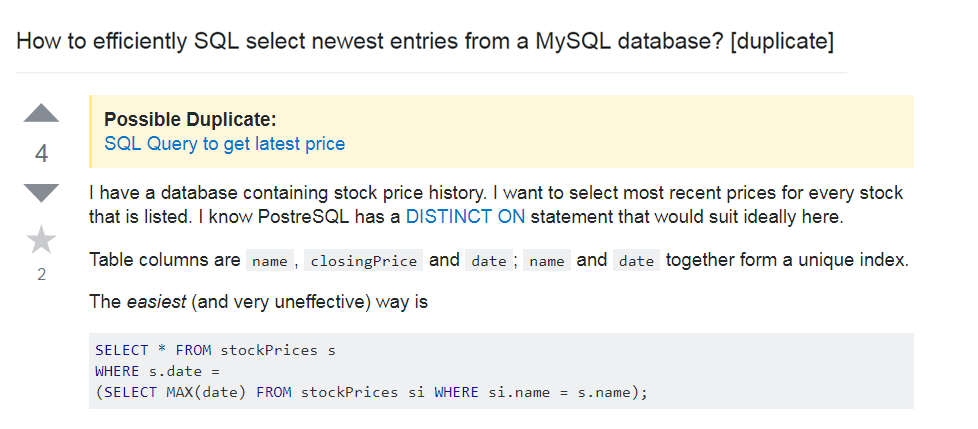
\includegraphics[width = 0.5\textwidth]{figures/duplicateex.png}
		\caption{Overview of the Main architecture}
		\label{fig:duplicateexample}
	\end{figure}
	But note that the same meaning may be expressed with totally different words, there is an example in Figure~\ref{fig:duplicateexample}
	So the traditional word-match based retrieval methods will not work in such cases.
	To overcome such semantic gap, we develop a neural-network based method to learn semantic of the sentences, so that it can spot semantic-similar questions in Stack Overflow.
	
	\begin{figure}
		\centering
		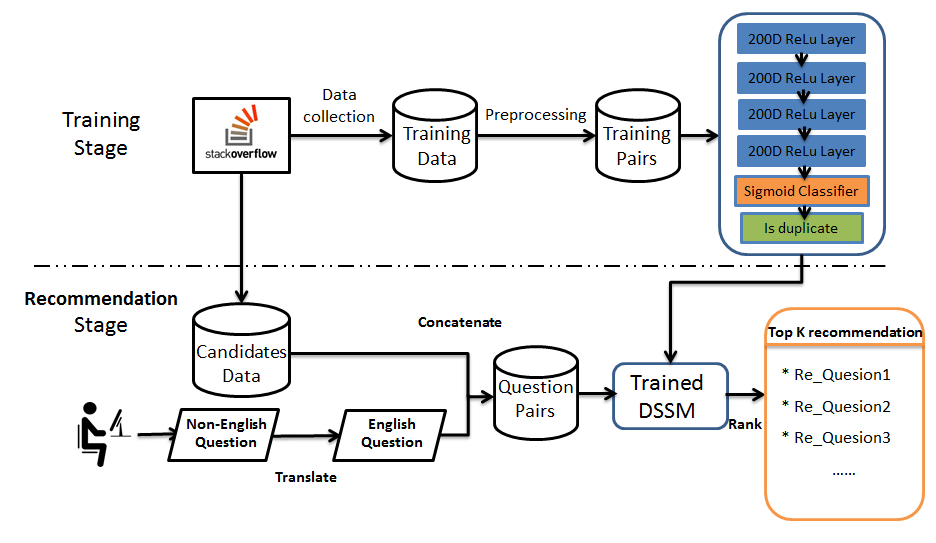
\includegraphics[width = 0.5\textwidth]{figures/model.png}
		\caption{Overview of the Main architecture}
		\label{fig:method}
	\end{figure}
	
	The overall architecture of the framework can be seen in Figure~\ref{fig:method} including training stage and recommendation stage.
	During the training phase, we obtain a deep semantic similarity model based on duplicated questions in Stack Overflow to overcome the semantic gap.
	Then, we translate the user's Russian query into English and then recommend related questions in Stack Overflow with the model. 
	More details can be seen below.
	
	%We consider the problem as a binary prediction one. Considering an input unit including a well-written title and a list of well-chosen tags, our approach uses the tags to filtering candidates and uses the title to predict and rank those candidates. The main architecture of the DSSM is illustrated in Figure 6. \par
	
	
	
	\begin{comment}
		First of all, we get the 310,000 pairs of duplicate questions from the Stack Overflow data dump[1] as the label for our model.	
		We then obtain the word embedding by training the whole Stack Overflow dataset.
		After that, we build the deep learning model by concatenating the duplicate question pair as input and train a similarity detection model with them.
	\end{comment}
	
	\subsection{Training Stage}	 
	 The overall approach is showed in Figure~\ref{fig:DSSM}.
	 We first collect duplicate question pairs as the training data. 
	 And then for each pair, we use RNN to encode the question title to a fixed-dimension vector.
	 After concatenating these two vectors, we train a fully-connected neural network to predict the score of their similarity.
	
	\begin{figure}[!h]
		\centering
		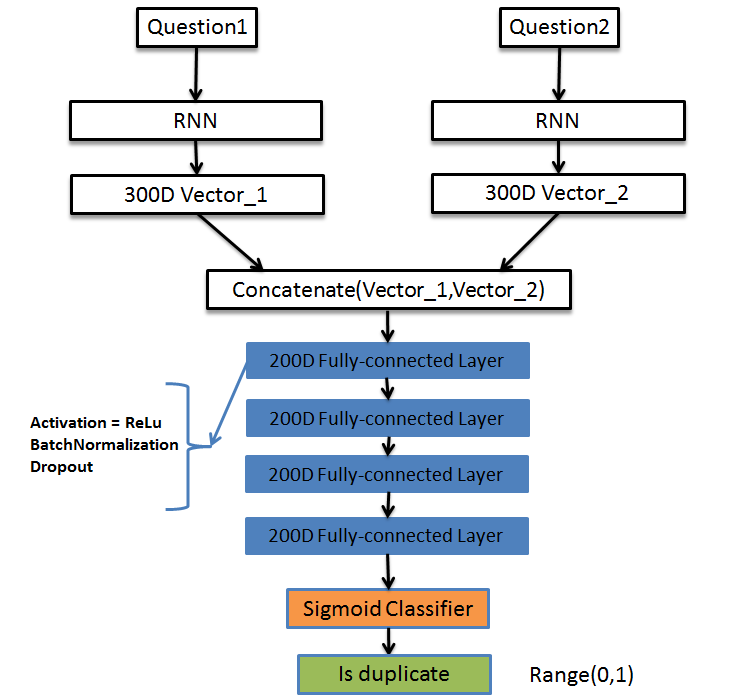
\includegraphics[width = 0.5\textwidth]{figures/modelac.png}
		\caption{Model architecture}
		\label{fig:DSSM}
	\end{figure}
	
	
	\subsubsection{Data collection}
	In Stack Overflow, thousands new questions are asked every day and there are tens of millions questions in total.
	Such a big corpus leads to the difficulty of searching, so sometimes, users may ask duplicate questions.
	Stack Overflow encourages users to mark such duplicates\footnote{https://stackoverflow.com/help/duplicates}, and then close them to help maintain the quality of the site.
	From the latest data dump, we locate 310,000 duplicate question pairs from post history and most of their titles are quite different but with the same meaning, according to our observation.
	For each pair of questions, we assume that their titles are semantically equivalent and then all of them are regarded as positive training data.
	Then we randomly sample the same-number of questions pairs to be the negative examples which are semantically different.
	So, we take merge these positive and negative question pairs as the data to train a model to detect semantic similarity of sentences. 
	 	
	\begin{comment}
	\subsection{Word Embedding}
	Mapping all the words into a dense low-dimensional vector space, words that appear in the similar sentence have a short distance in the embedding space, and each dimension represents a latent semantic [13,14]. The assumption is that words appeared in the similar context have similar meanings, so their mapped vectors in the embedding vector space should be relatively close. Word embedding only needs a large amount of text to learn as it is an unsupervised method. 
	\par 
	For example, given an English duplicate question pairs, the word embedding system will convert it into embedding space by mapping each word with the dictionary of words after preprocessing.  Then, concatenating the two vectors as a unit, it will be the input of the deep learning model.
	\end{comment}
	
	\subsection{RNN}
	
	\begin{figure}[!t]
		\centering
		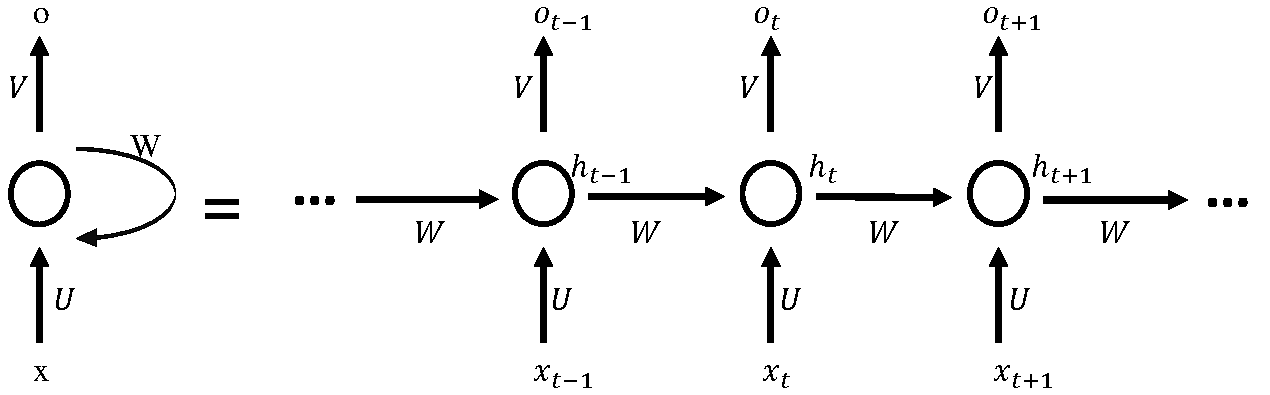
\includegraphics[width=0.45\textwidth]{figures/rnn.pdf}
		\caption{Recurrent Neural Network}
		\label{fig:rnn}
	\end{figure}
	
	Recurrent Neural Network (RNN) is a class of neural networks where connections between units form directed cycles.
	Due to its nature, it is especially useful for tasks involving sequential inputs such as speech recognition~\cite{graves2013speech} and code completion~\cite{white2015toward}.
	Compared with traditional n-gram language model, a RNN-based language model~\cite{mikolov2010recurrent} can predict a next word by preceding words with variant distance rather than a fixed number of words.
	
	As shown in Figure~\ref{fig:rnn}, the architecture of a basic RNN model includes three layers.
	An input layer maps each word to a vector such using word embedding or one-hot word representation.
	A recurrent hidden layer recurrently computes and updates a hidden state after reading each word.
	An output layer estimates the probabilities of the next word given the current hidden state.
	Figure~\ref{fig:rnn} shows the unfolding in time of the computation in RNN's forward computation.
	we put the question title into the RNN and take the last state (a vector) of the RNN model as its semantic.
	
	\subsubsection{Similarity Detection Model}
	After getting the vector from RNN, we concatenate two vectors of the question pairs into a long vector.
	Then this vector will pass four-layer fully-connect neural network.
	Note in each layer, we carry out a batch normalization~\cite{??} and dropout\cite{??} to avoid overfitting.
	And we select $ReLu$~\cite{??} as our activation function which is widely used in deep learning works due to its similarity to signal processing in human brain:
	\begin{equation}
		ReLu(i) = \max(0, i)
	\end{equation}
	For the input less than one, it will output 0, otherwise preserve the input value.
	The last layer of the model is to take the sigmoid activation function to predict if the question pair is semantically same or different.
	As we formulate this question into binary classification, we adopt cross entropy as the loss function.
	During training, the parameters within the model are learned by backpropagation~\cite{werbos1990backpropagation} with gradient descent to minimize the error rate.
	After training, given two questions, it will not only predict if they are semantically same or not, but also return the probability of it. 
	Such probability represents the confidence of the model.
	
	\begin{comment}
		Figure~\ref{fig:DSSM} \textcolor{red}{For the figure, please use the ref command.} presents the architecture of our deep semantic similarity model(DSSM), which is based on the Stanford Natural Language Inference [16]. This model takes a vector pair of embedded questions as input. Firstly, tokenize the two questions into word sequence then process the word embedding. We need to add padded dimensions to keep all embedding sentences in the same shape (assume each sentence vector has 25 dimensions). Also, we use the GloVe the form a Weight matrix Rw t*Dw that t is the total words number and Dw is the max dimension number of the embedding (assume Dw is 300). 
	\end{comment}
	
	\par
	
	\begin{comment}
	we choose the $relu$ activation function because of its performance better than other activation functions in the one hot vector calculation. Also, we determine to use sigmoid as the activation function in the bottom layer because the sigmoid activation function is better for the binary classification problem. Our approach also adopts the Batch normalization algorithm[17] that can faster the learning speed and higher overall accuracy. There are four fully connected layers which dense is 200 and use dropout to overcome the overfitting problem.
		\par
		For the last layer, the DSSM should output a parameter called is\_duplicate that range from 0 to 1, which indicates the similarity of the input question pair. We use the sigmoid activation function and binary cross entropy for this binary classification problem.
		\par
	\end{comment}
	 
	

	
	\subsubsection{Implementation}
	In this paper, we first tokenize the question titles and then train a model~\cite{??} on that corpus and convert each word into a vector with 300 dimension.
	Slightly different from the basic RNN above, we adopt a more advanced RNN called LSTM (Long short-term memory)~\cite{??} which is more powerful to capture the semantic of long sentences.
	There are 256 nodes in the LSTM model, and as the input word is 300dim vector, the last hidden state is also a 300dim vector.
	We develop the model based on Keras~\cite{??}, and the model is trained by 25 epochs (i.e., iterating all data 25 times).
	\begin{comment}
	In this paper, we use the Keras tokenizer to tokenize all the questions in the training data set that we mined from the raw data. We also adopt GloVe, which is a popular word embedding tool. For the embedding space, each dimension represents a latent semantic feature of a word. We get a dictionary of all the word that appeared in the text, and finally, there are 0.21 million dimensions in the embedding space.
	\end{comment}
	 
	
	
	\subsection{Recommendation stage}
	After we got the model, we can use it to recommend Stack Overflow questions according to their query.
	The users in Russian Stack Overflow will send a query to the model in Russian language.
	We first translate it into English with Google Translate.
	As our model can only detect the similarity of two questions, we then compare the query with all questions in our database.
	For each question, we obtain a score indicating how much the question is related to the query.
	Then we sort all questions in database based on their scores in decent and recommend top 10 of them to the users.
	Note the translated sentence may not be perfect, but as our semantic similarity model is capable tp bridge the semantic gap, it can still return reasonable results.
	